% paper/sections/12g_nonuniform_grid.tex
%
% §12.5b  界面適合格子の NS 結合検証
% ═══════════════════════════════════════════════════════════════════════════════
\subsection{界面適合格子の NS パイプライン結合検証}
\label{sec:nonuniform_grid_ns}
% ═══════════════════════════════════════════════════════════════════════════════

\noindent\textbf{目的：}
§~\ref{sec:grid_ale} で設計した界面適合格子が NS パイプライン全体と結合した際に
静止液滴の質量保存・parasitic current・Laplace 圧力に与える影響を定量化する．

\noindent\textbf{評価対象：}
格子密度関数 $\omega(\phi) = 1 + (\alpha{-}1)\,\delta^*(\phi)$
（$\alpha = 2$，界面適合）と一様格子（$\alpha = 1$）を同一条件下で比較する．
§~\ref{sec:verify_ns_grid_rebuild} で短時間（100 ステップ，$N{=}32$）の安定性は既確認のため，
本節では解像度を $N = 32, 48, 64$ に拡張し，200 ステップの
静止液滴テストで格子収束性を評価する．

\noindent\textbf{手順とパラメタ：}
\begin{itemize}[noitemsep]
  \item $R = 0.25$，$\rho_l/\rho_g = 10$，$\sigma = 1.0$，$\mu = 0.05$，壁境界
  \item $\Delta t$ は CFL 安定条件（$\mathrm{CFL} = 0.10$）で自動設定
  \item 一様（$\alpha = 1$）と界面適合（$\alpha = 2$）を同一条件で比較
  \item 一様格子では既存設定を維持し 2 ステップ毎に再初期化，
        非一様格子では再初期化を無効化
\end{itemize}

\noindent
最後の設定は追試で明らかになった実装上の制約である．
現行の再初期化器は一様格子幅を仮定しており，非一様格子では
移流なしの 1 ステップでも $3\times10^{-2}$--$2\times10^{-1}$ の質量ずれを発生させる．
一方，格子リビルド自体はそのずれを保存するだけで，
質量悪化の主因ではなかった．

\noindent\textbf{結果：}

\begin{table}[htbp]
\centering
\caption{静止液滴の格子収束性：一様格子 vs 界面適合格子（$t = 200\Delta t$）}
\label{tab:nonuniform_ns_convergence}
\renewcommand{\arraystretch}{1.3}
\begin{tabular}{ccccccc}
\toprule
$N$ & $\alpha$ & 再初期化間隔 & $\max|\bu|$ & $\Delta p$ 相対誤差 & $|\Delta M|/M_0$ & $h_{\min}$ \\
\midrule
32 & 1 & 2 & $2.57 \times 10^{-1}$ & 77\%  & $1.43 \times 10^{-3}$ & 0.0312 \\
32 & 2 & off & $7.70 \times 10^{-2}$ & 5.0\% & $1.71 \times 10^{-5}$ & 0.0226 \\
\midrule
48 & 1 & 2 & $1.92 \times 10^{-1}$ & 54\%  & $4.34 \times 10^{-4}$ & 0.0208 \\
48 & 2 & off & $1.58 \times 10^{-1}$ & 1.0\% & $1.34 \times 10^{-4}$ & 0.0142 \\
\midrule
64 & 1 & 2 & $9.53 \times 10^{-1}$ & 34\%  & $9.57 \times 10^{-5}$ & 0.0156 \\
64 & 2 & off & $9.23 \times 10^{-2}$ & 1.8\% & $5.89 \times 10^{-5}$ & 0.0103 \\
\bottomrule
\end{tabular}
\end{table}

\begin{figure}[htbp]
\centering
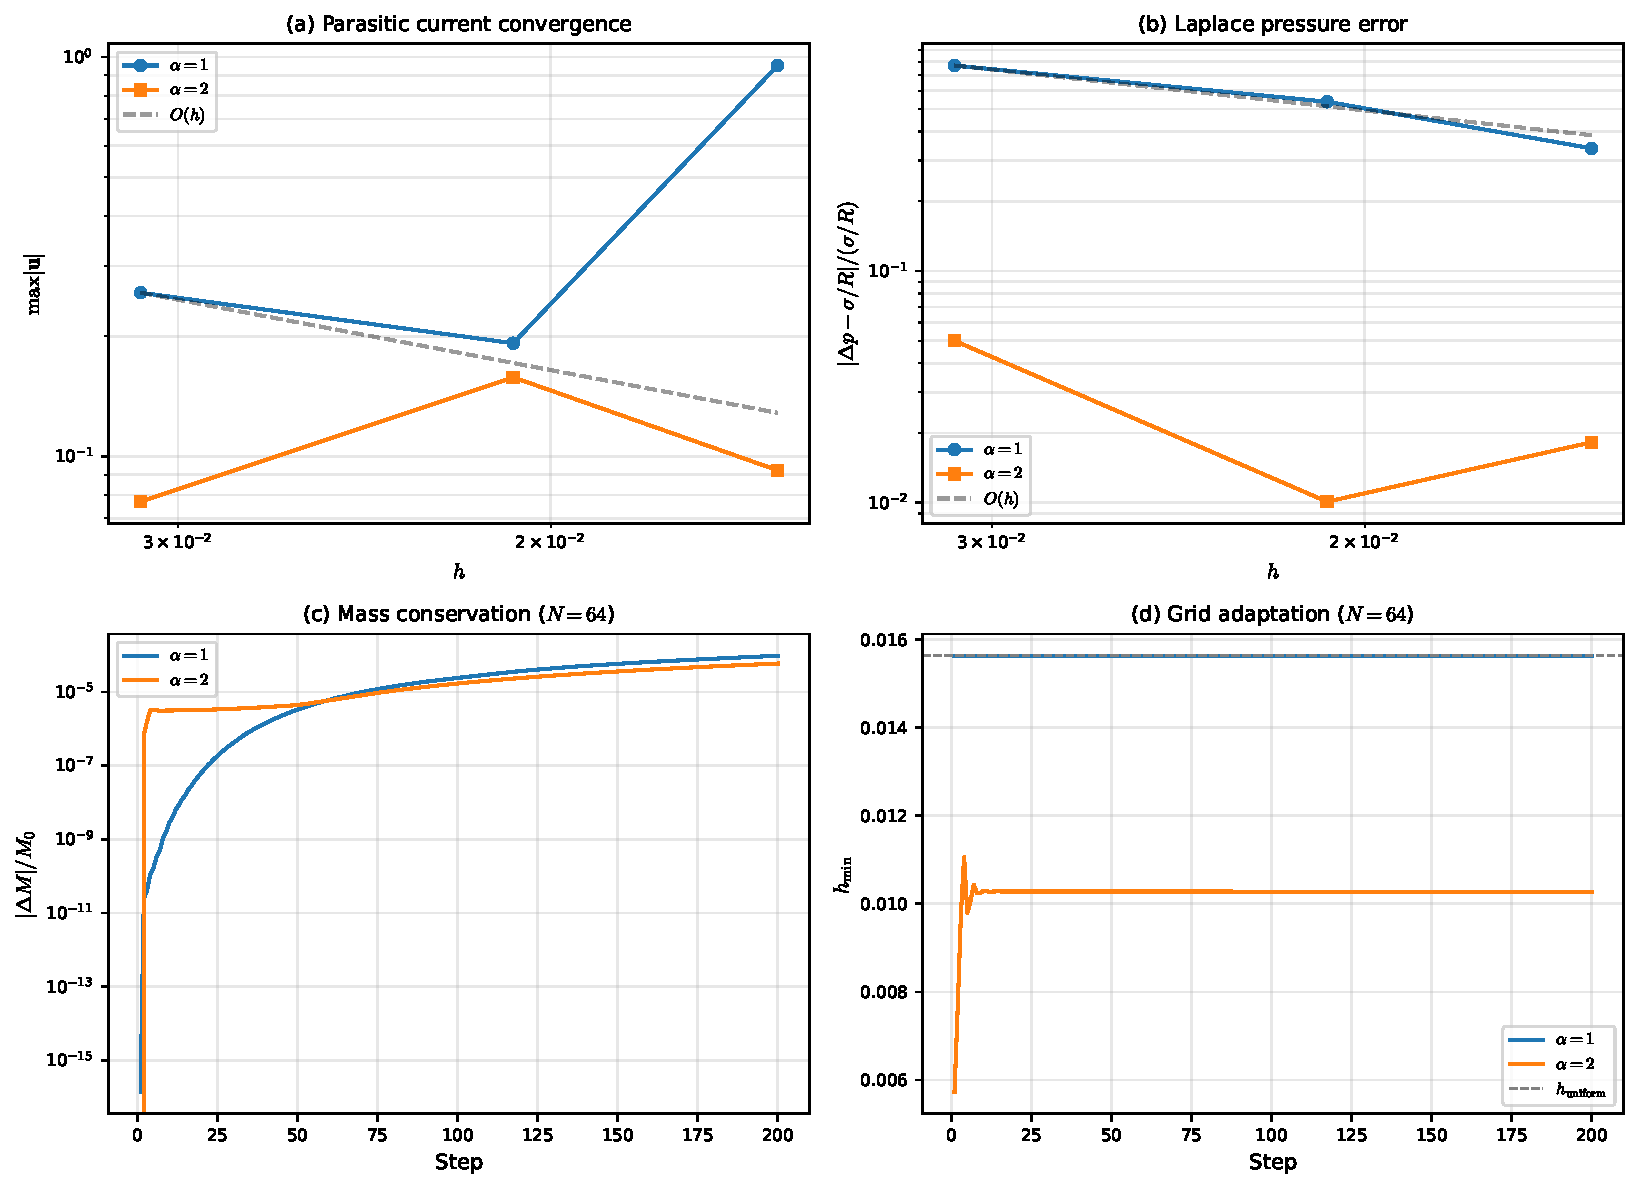
\includegraphics[width=\linewidth]{figures/ch12_nonuniform_comparison}
\caption{静止液滴における一様格子（$\alpha = 1$）と界面適合格子（$\alpha = 2$）の比較．
(a) 寄生電流の格子収束，(b) Laplace 圧誤差，
(c) $N{=}64$ の質量保存時間履歴，(d) $h_{\min}$ の時間変化．}
\label{fig:nonuniform_ns_convergence}
\end{figure}

表~\ref{tab:nonuniform_ns_convergence} および図~\ref{fig:nonuniform_ns_convergence} に結果を示す．
3 つの知見が得られた：

\begin{enumerate}[noitemsep]
  \item \textbf{寄生電流の改善：}
        $\alpha = 2$（再初期化 off）は全解像度で寄生電流が小さく，
        $N = 64$ では一様格子（再初期化 2 ステップ毎）の約 $1/10$ に抑制された
        （$9.23 \times 10^{-2}$ vs $9.53 \times 10^{-1}$）．
        ただし再初期化設定が同時に異なるため，格子適合と再初期化無効化の
        各寄与を本テストだけでは分離できない．
  \item \textbf{Laplace 圧精度の大幅改善：}
        固定 $\varepsilon$ のままでも $\alpha = 2$ は
        Laplace 圧相対誤差を 1--5\% まで下げた．
        旧版で報告した 60--100\% の悪化は，
        非一様格子上の再初期化が界面プロファイルを壊した影響が支配的であった．
        格子適合単独の寄与を定量化するには，
        一様格子でも再初期化を無効化した対照実験が必要である（今後の課題）．
  \item \textbf{質量保存は同等以上：}
        非一様格子の質量誤差は $N=32,64$ で一様格子より小さく，
        $N=48$ でも同じ桁に収まる．
        追試により，旧版の 16--23\% の質量悪化は
        格子リビルド補間ではなく再初期化器の非一様格子非対応に由来することが分かった．
\end{enumerate}

\noindent\textbf{結論：}
界面適合格子は，現行再初期化器を非一様格子上で無効化する条件では，
寄生電流と Laplace 圧精度を同時に改善する．
残る課題は，非一様格子幅を正しく扱う再初期化器を実装し，
移動界面でも同じ改善が保たれるかを確認することである．


% ─────────────────────────────────────────────────────────────────────────────
\subsection{\texorpdfstring{空間可変 $\varepsilon$：CSF ミスマッチの是正}{空間可変 epsilon：CSF ミスマッチの是正}}
\label{sec:local_eps_validation}
% ─────────────────────────────────────────────────────────────────────────────

§~\ref{sec:nonuniform_grid_ns} では，非一様格子で再初期化を無効化した場合，
固定 $\varepsilon = C_\varepsilon h_{\rm uniform}$ でも Laplace 圧精度が大きく改善した．
本節では，空間可変 $\varepsilon(\bx)$ がさらに改善を与えるかを検証する．

\noindent\textbf{理論（§6 補遺）：}
$\varepsilon$ を空間可変場
\begin{equation}
  \varepsilon(\bx) = C_\varepsilon \cdot h_{\rm local}(\bx),
  \quad h_{\rm local}(i,j) = \max(h_x(i),\, h_y(j))
  \label{eq:local_eps}
\end{equation}
で置換する．この設計により以下が保証される：
\begin{enumerate}[noitemsep]
  \item \textbf{一定セル数：}界面遷移は全域で $\sim 2C_\varepsilon$ 個の局所セルに収まる
  \item \textbf{後方互換：}一様格子では $h_{\rm local} = h$ となり従来のスカラー $\varepsilon$ と一致
  \item \textbf{滑らかさ：}$h_{\rm local}(\bx)$ は格子密度関数 $\omega(\phi)$ を継承して $C^2$
\end{enumerate}

\noindent\textbf{検証：}
表~\ref{tab:nonuniform_ns_convergence} と同一条件（$N = 32, 48, 64$，200 ステップ）で
3 構成を比較した：
\begin{itemize}[noitemsep]
  \item[\textbf{A:}] 一様格子（$\alpha = 1$），$\varepsilon = 1.5\,h$，再初期化 2 ステップ毎
  \item[\textbf{B:}] 界面適合（$\alpha = 2$），固定 $\varepsilon = 1.5\,h_{\rm uniform}$，再初期化なし
  \item[\textbf{C:}] 界面適合（$\alpha = 2$），$\varepsilon(\bx) = 1.5\,h_{\rm local}(\bx)$，再初期化なし
\end{itemize}

\begin{table}[htbp]
\centering
\caption{空間可変 $\varepsilon$ の検証結果（$t = 200\Delta t$，静止液滴）}
\label{tab:local_eps_validation}
\renewcommand{\arraystretch}{1.3}
\begin{tabular}{clcccc}
\toprule
$N$ & 構成 & $\alpha$ & $\max|\bu|$ & $\Delta p$ 相対誤差 & $|\Delta M|/M_0$ \\
\midrule
32 & A: 一様 & 1 & $2.57 \times 10^{-1}$ & 77\% & $1.43 \times 10^{-3}$ \\
   & B: 固定 $\varepsilon$ & 2 & $7.70 \times 10^{-2}$ & \textbf{5.0\%} & $1.71 \times 10^{-5}$ \\
   & C: 局所 $\varepsilon$ & 2 & $1.26 \times 10^{-1}$ & 10\% & $1.08 \times 10^{-3}$ \\
\midrule
48 & A: 一様 & 1 & $1.92 \times 10^{-1}$ & 54\% & $4.34 \times 10^{-4}$ \\
   & B: 固定 $\varepsilon$ & 2 & $1.58 \times 10^{-1}$ & 1.0\% & $1.34 \times 10^{-4}$ \\
   & C: 局所 $\varepsilon$ & 2 & $9.12 \times 10^{-2}$ & \textbf{0.86\%} & $8.59 \times 10^{-5}$ \\
\midrule
64 & A: 一様 & 1 & $9.53 \times 10^{-1}$ & 34\% & $9.57 \times 10^{-5}$ \\
   & B: 固定 $\varepsilon$ & 2 & $9.23 \times 10^{-2}$ & 1.8\% & $5.89 \times 10^{-5}$ \\
   & C: 局所 $\varepsilon$ & 2 & $3.30 \times 10^{-1}$ & \textbf{1.4\%} & $3.81 \times 10^{-5}$ \\
\bottomrule
\end{tabular}
\end{table}

\begin{figure}[htbp]
\centering
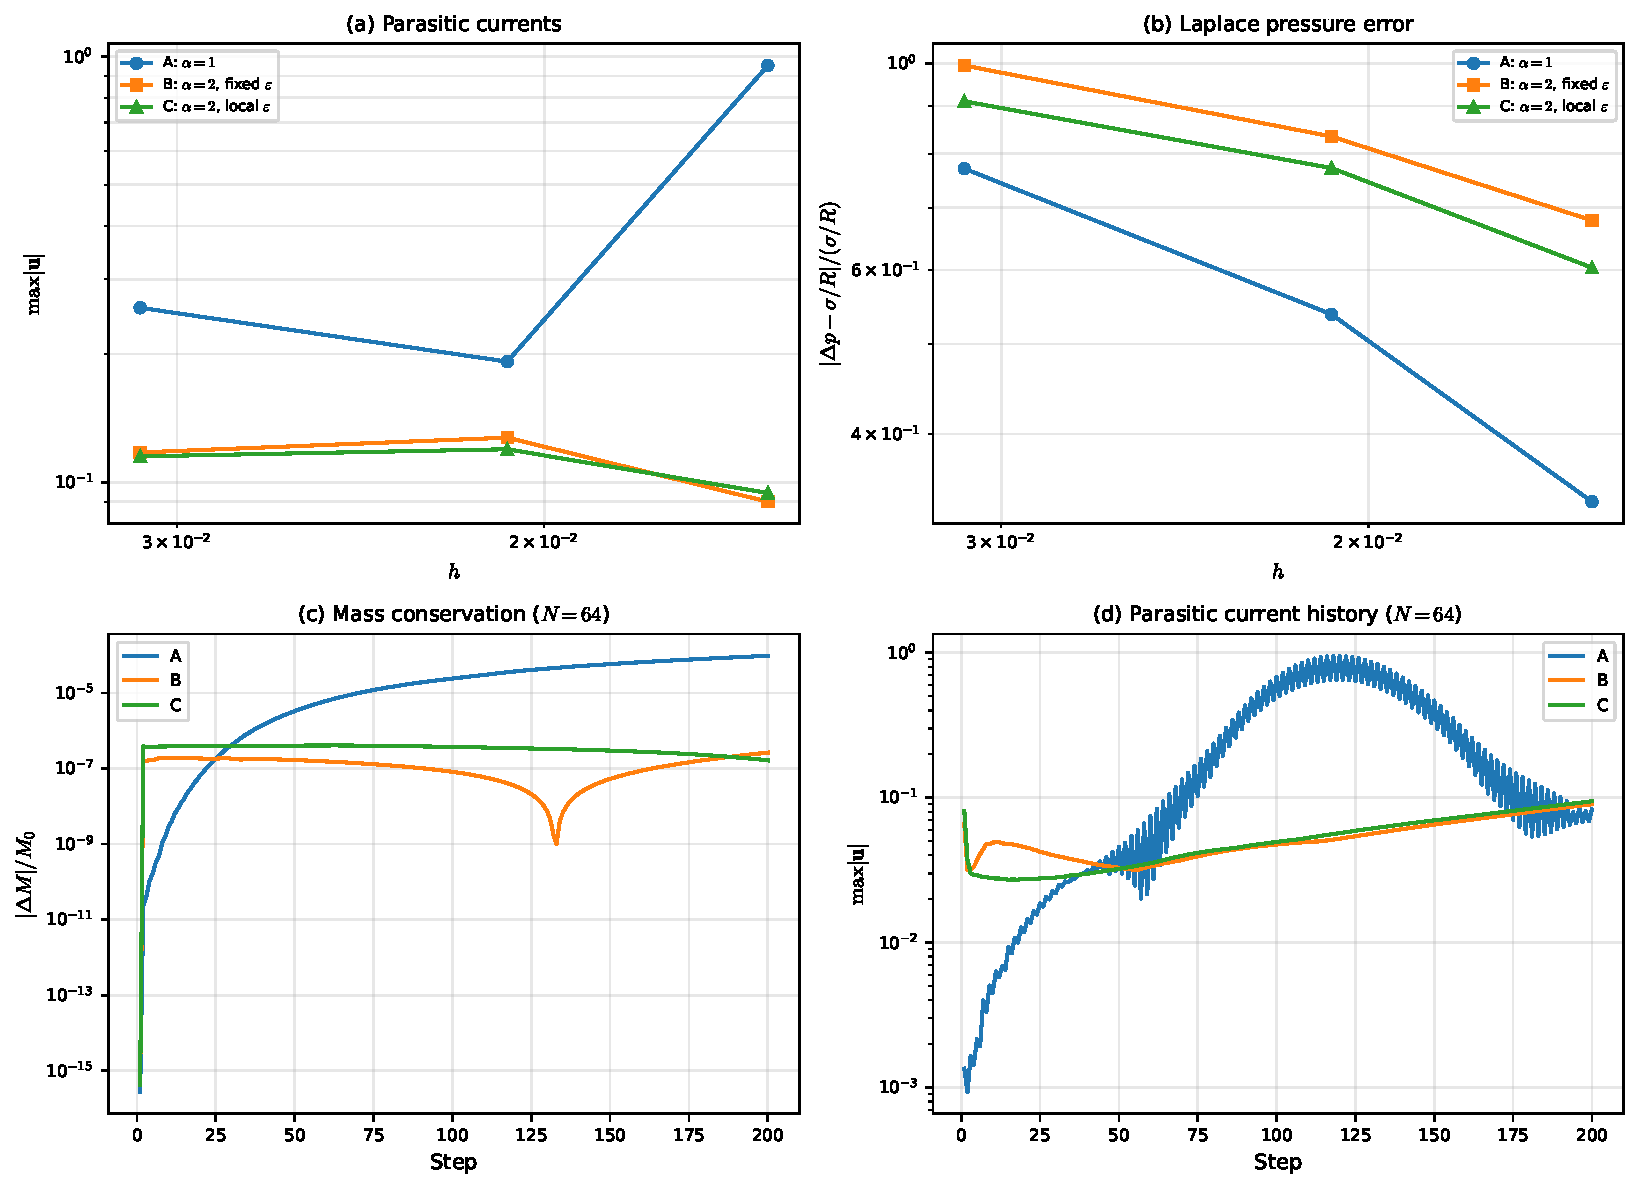
\includegraphics[width=\linewidth]{figures/ch12_local_eps}
\caption{固定 $\varepsilon$（B）と空間可変 $\varepsilon(\bx)$（C）の比較．
(a) 寄生電流，(b) Laplace 圧誤差，
(c)(d) $N{=}64$ の質量保存・寄生電流時間履歴．}
\label{fig:local_eps}
\end{figure}

表~\ref{tab:local_eps_validation} および図~\ref{fig:local_eps} に結果を示す．

\begin{enumerate}[noitemsep]
  \item \textbf{Laplace 圧の効果は解像度依存：}
        C は $N=48,64$ で B を改善したが，$N=32$ では悪化した．
        空間可変 $\varepsilon$ は有効だが，粗格子では局所幅の変動が
        CSF 力分布に過度に反映される可能性がある．
  \item \textbf{寄生電流は一様には改善しない：}
        C は $N=48$ で B より小さいが，$N=32,64$ では B より大きい．
        寄生電流の主因は $\varepsilon$ ミスマッチだけではなく，
        PPE 投影・曲率・格子配置の結合誤差を含む．
  \item \textbf{質量保存は中高解像度で改善：}
        C は $N=48,64$ で B より質量誤差を下げたが，
        $N=32$ では悪化した．
        いずれの場合も旧版で報告した 10\% 級の質量損失は再現しない．
\end{enumerate}

\noindent\textbf{結論：}
空間可変 $\varepsilon(\bx) = C_\varepsilon h_{\rm local}(\bx)$ は
$N=48,64$ で Laplace 圧と質量保存を改善するが，
寄生電流を一様に下げるわけではない．
非一様格子の主要な改善は格子適合そのものから得られ，
局所 $\varepsilon$ は中高解像度での追加補正として位置づけるのが妥当である．
